\chapter{Volumetric Zoning}
\label{ch:Volumetric Zoning}

\begin{figure}[h] \centering
	\adjustbox{trim={.25\width} {.0\height} {.25\width} {.0\height},clip}%
	{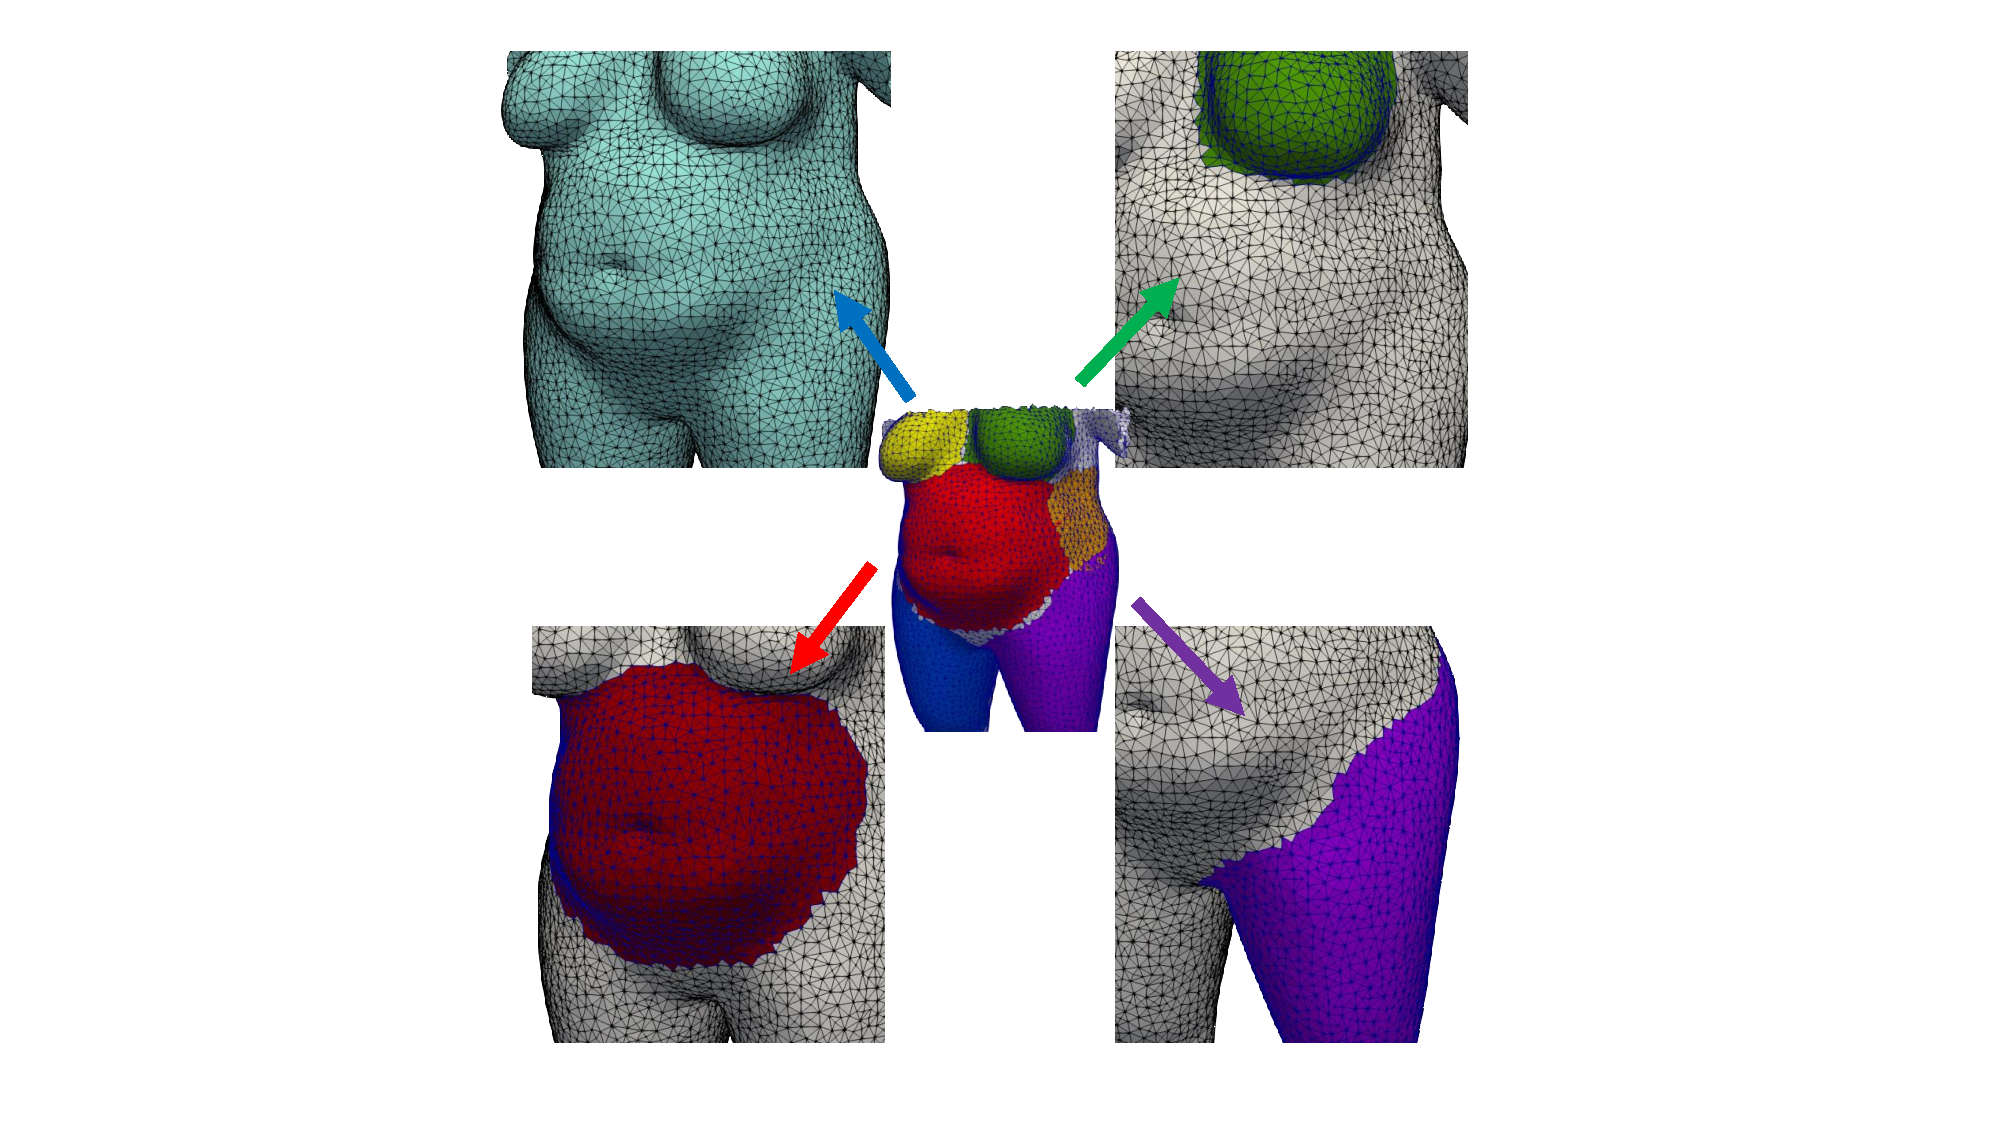
\includegraphics[width=6.0in]{images/body_xl/zones.pdf}}
	\caption{\textbf{Body Zones}: Volume preserving zones on the body mesh used for simulation in
		Figure~\ref{fig:teaser}. Six significant anatomical compartments (belly (red), side and back waist (orange), 2 legs (blue and purple), 2 breasts (yellow and green)) are selected as zones. Additionally, another zone is added including the full body (cyan), so that the entire body would be volume preserving. Note that the full body zone is not necessary, but can be added to ensure the volume preservation of not only each compartments but also the entire body. The zones are drawn on the mesh surface with a texture painting tool in a visual effects software, and then projected to the inner body using our projection method. }
	\label{fig:body_zones}
\end{figure}

For a more complete description of the pipeline, we propose a simple method of obtaining
volumetric zones on a tetrahedral mesh from surface vertex annotation.

Manual vertex painting is a very common part of
many character animation pipelines, allowing users to assign attributes such as skinning weights.
Alternatively, there are methods to automatically compute transformation weights from
skeleton meshes \cite{Rohmer:2009, Baran:2007, Weber:2007}, from sparse subsets of degrees of freedom
\cite{Jacobson:2012}, or from animation data \cite{James:2005}. 

Using either of the aforementioned methods, we end up with a set of weights defining possibly
overlapping zones on the surface of our FEM mesh. We then transfer this data onto the surface
triangles. Naturally these surface zones should be simply connected in order for the volumetric
zones to follow suit.

In order to transfer zone information to the rest of the tetrahedral mesh, we first construct a
smooth potential field around the mesh surface using Hermite Radial Basis Functions
\cite{Pai:2018, Vaillant:2013, Macedo:2009, Wendland:2004}, although any signed distance field will
do.  We then project each tetrahedron centroid along the potential gradient onto the surface
triangles. The triangle zone information is then copied from the triangles, back to the
source tetrahedra.

Albeit simple, this projection is an effective method to map internal tetrahedral mesh elements to
surface triangles. This way, we allow the users to define volume preserving zones by simply
painting surface vertices with any existing tool. We demonstrate
this approach with an sample female body simulation mesh on Figure~\ref{fig:body_zones}, where the
surface zones are chosen manually to capture the anatomical volume-preserving regions. 